\documentclass{article}
\usepackage{amssymb, amsfonts, amsmath, geometry, verbatim, caption}
\geometry{letterpaper}
\usepackage[parfill]{parskip}    		
\usepackage{graphicx}
\graphicspath{{./}}
\usepackage[nottoc,numbib]{tocbibind}
\usepackage[utf8]{inputenc}

\usepackage{listings}
\usepackage{xcolor}

\definecolor{codegreen}{rgb}{0,0.6,0}
\definecolor{codegray}{rgb}{0.5,0.5,0.5}
\definecolor{codepurple}{rgb}{0.58,0,0.82}
\definecolor{backcolour}{rgb}{0.95,0.95,0.92}

\lstdefinestyle{mystyle}{
    backgroundcolor=\color{backcolour},   
    commentstyle=\color{codegreen},
    keywordstyle=\color{magenta},
    numberstyle=\tiny\color{codegray},
    stringstyle=\color{codepurple},
    basicstyle=\ttfamily\footnotesize,
    breakatwhitespace=false,         
    breaklines=true,                 
    captionpos=b,                    
    keepspaces=true,                 
    numbers=left,                    
    numbersep=5pt,                  
    showspaces=false,                
    showstringspaces=false,
    showtabs=false,                  
    tabsize=2
}

\lstset{style=mystyle}


\newcommand{\R}{\mathbb{R}}

\title{Calculating the Solvent Exposed Surface Area of Proteins with Intersecting Spheres} 
\author{Gargi Kher, Neil Gupta}
\date{\today}

						
\begin{document}

\maketitle
\tableofcontents
\newpage
\section{Abstract}
Calculating the solvent-exposed surface area (SASA) of large biomolecules is an important problem in structural biology, especially in the case of proteins, where small changes in the molecule's shape can greatly limit the protein's ability to do its job. The fraction of a polar atom's surface area that is exposed to the engulfing solvent can be the difference between a stable hydrogen bond being formed with the solvent and a polar atom buried within the protein, which could prevent the protein from folding into its proper shape. Molecular dynamics simulations, which use computers to predict the time evolution of a molecular system also rely on accurate SASA calculations as a way to compute the enthalpy of hydration for the molecules in the system. Today, SASA is usually calculated based on an implicit solvation model, where the solvent is taken to be a continuous field that the molecules of interest sit in. The atoms are taken to be spheres of definite radius, and thus calculating the SASA of an atom involves calculating the fraction of the sphere that is exposed. The SASA of the entire molecule can be found by summing this quantity over all atoms. This paper gives a overview of \textsc{alphamol}, a way of analytically calculating the derivative of SASA with respect to time, a quantity which can be numerically integrated as part of a molecular dynamics simulation to predict the future state of a molecular system. The chief benefits over other algorithms are numerical stability and an ability to consider internal atoms, which older SASA calculators sometimes ignored.\cite{Bryant} We also discuss two previous ways of computing SASA that \textsc{alphamol} improves upon. Finally we do some calculations of our own to benchmark the performance of these two methods and provide some modern context for where SASA computations are used.

\section{Previous Work}
Accurately and quickly calculating the SASA of proteins has been a problem that people have been trying to solve since the 1980's. One reason for this is the fact that the effective potential for solvation can be written $W=W_{elec}+W_{np}$, where $W_{elec}$ represents the electrostatic contribution and $W_{np}$ represents the nonpolar contribution to this potential. The second term depends heavily on the SASA value of the polar atoms in the molecule, as polar atoms with a low SASA value (buried polars) should to make internal hydrogen bonds to preserve the protein's structure. One of the earliest ways of computing this value was by Richmond (1984). His method involved modeling atoms as spheres and computing SASA as an application of the Gauss-Bonnet Theorem. This method was the basis for many future SASA calculators that optimized for attributes like speed or numerical stability. Other methods didn't focus as much on exact values in the interest of speed. The Shrake-Rupley algorithm (optimized by Legrand and Merz as discussed below), breaks up the spherical surface of each atom into a set of dots, and uses the fraction of dots that are exposed as a proxy for the exposed surface area. This is the default SASA calculator in Rosetta, a software package developed at the UW that allows for the computational analysis and design of protein structures. 
\subsection{Geometrical Representation of Atoms}
While atoms are comprised of protons, neutrons, and electrons, electrons are what give them their properties. Electrons make up the volume of an atom, and are generally found near the nucleus. Because we don’t know for certain where electrons are in an atom, their positions are represented by orbitals, which give the probability of electrons being in a particular location. Orbitals can take on different shapes, generally resembling some type of dumbbell, but when they come together, they form a roughly spherical shape (DeCoste, Zumdahl p.551-557). This is why atoms are often mathematically modeled as spherical objects.
\subsection{The Shrake-Rupley Algorithm}
The Shrake-Rupley Algorithm (Shrake and Rupley, 1973) is the standard way of calculating SASA by approximating the surface as a discrete set of voxels instead of a continuous surface. This can lead to inaccuracies, but the gains in speed are usually worth it. The algorithm can also fail if the protein surface is not continuous (i.e. an internal cavity is present) or the atomic radii are too small. This algorithm, once optimized by Legrand and Merz (1993) became a standard SASA calculator. Comparing this algorithm with the analytic SASA calculator MSEED (Perrot et al.) in calculating the SASA of the protein BPTI showed Shrake-Rupley to be roughly six times faster than MSEED, a huge improvement. The method works by representing the surface of sphere $a_i$ by an array of $l$ points evenly distributed on the surface of a sphere of radius $r_i$. The exposed surface area of $a_i$ can be written as
\begin{equation}
A_i=4\pi r_i^2\frac{l_{exposed}}{l_{total}} 
\end{equation}
where $l_{exposed}$ is the number of points that are solvent exposed. Now if we were to calculate this quantity for each atom we would need to make $nkl$ calculations, where $k$ is the average number of atoms that intersect a given atom. This could get quite intensive. What Legrand and Merz did was realize that any surface point is either buried or exposed, and thus the state of $a_i$'s surface points could be represented as an $l/8$ byte string $b_i$, where $b_{ij}=1$ means that the point is exposed and $b_{ij}=0$ means that the point is buried. This has the benefit of making the calculation of the points on $a_i$ buried by a neighboring sphere $a_q$ a boolean AND operation on $b_i$. By defining $m_{iq}$ as a boolean string with $k^{th}$ element 0 when the $k^{th}$ point of sphere $a_i$ is buried by $a_q$ and 1 otherwise, the set of points on $a_i$ left exposed by the intersection with $a_q$ is (111...1) \& $m_{iq}$. Thus 
\begin{equation*}
b_i=(111...1) \text{ \& } m_{i1} \text{ \& } m_{i2} \text{ \& } m_{i3} \text{ \& }...\text{ \& } m_{ik} \text{ \& } m_{ik+1}
\end{equation*}
for each $a_k$ that intersects $a_i$.
The SASA of $a_i$ can then be calculated by $(1)$ by setting $l_{exposed}$ as the number of bits in $b_i$. \par
To actually calculate $m_{iq}$, we first compute 
\begin{align}
&\cos\theta_{iq}=\frac{r_i^2+r_{iq}^2-r_q^2}{2r_ir_{iq}} \\
&d_{iq}=2r_i\sin\theta_{iq}=2r_i\sqrt{\frac{1-\cos\theta_{iq}}{2}}=r_i\sqrt{2(1-\cos\theta_{iq})}
\end{align}

\begin{figure}
\caption{Calculation of $d_{iq}$ and $\theta_{iq}$ for the purpose of calculating $m_{iq}$.}
\centerline{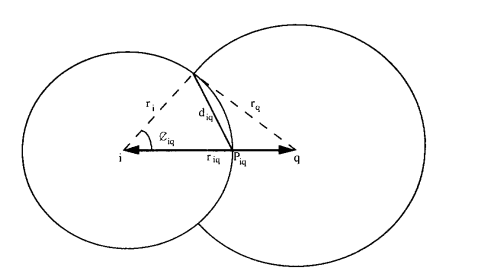
\includegraphics[width=3in]{mask}}
\end{figure}

All points on $a_i$ within $d_i$ of the $P_{iq}$ are buried, and those bits in $m_{iq}$ are set to zero, with the rest set to 1. This string can be AND'ed with $b_i$ to produce a new $b_i$. This can be done for all spheres that intersect $a_i$ for each sphere in turn. The key insight that cuts down on the $nkl$ calculations is the fact that the $m_{iq}$ can be stored and retrieved later if the same string is ever needed. This is very likely to occur, because the $d_{iq}$ can be made independent of $r_i$ by removing the factor $r_i$. Then $d_{iq}=\sqrt{2(1-\cos\theta_{iq})}$. Now we can calculate $m_{iq}$ for the range of $d_{iq}$ from 0-2. Once we store these masks, we will have covered all possible overlaps between spheres because we have gone through all angles $\theta_{iq}$.
This provides a method of calculating the SASA of the entire protein. We can simply look at every intersection with a given atom and lookup the appropriate mask (based on the angle $\theta_{iq}$. Then we scale it by the radius of the atom we are looking at. Then we can perform our AND operations and find the SASA for a given atom. Iterating over all atoms gives us our answer.
\subsection{Richmond's Algorithm and the Gauss-Bonnet Theorem}
In a previous paper written by Richmond (1984), a different strategy is used to find the solvent exposed surface area of the atoms. He still represents the atoms as spheres with definite radius with centers at the atomic coordinates, but instead of using voxels, he made use of the Gauss-Bonnet theorem, a fundamental theorem in differential geometry which connects the topological properties of a manifold (specifically its Euler Characteristic) with its geometric properties (its curvature). A standard statement of the theorem is 

\begin{equation}
\int_M KdA + \int_{\partial M} k_g ds = 2\pi\chi(M)
\end{equation}
Here $\chi$ is the Euler Characteristic of $M$, and $K$ and $k_g$ are the Gaussian and geodesic curvatures of the manifold and the boundary respectively. For polygons, $\chi=V-E+F=1$. 

The SASA of an atom with radius $\varrho_i$ lies on a sphere where $K=\frac{1}{\varrho_i^2}$. We can divide this SASA into many polygons bounded by the circles of intersection with neighboring spheres (See Figure 2). If $M$ is one particular region of that SASA, we can write 
\begin{align}\nonumber
&\frac{1}{\varrho_i^2}\int_M dA + \int_{\partial M} k_g ds= 2\pi \\
&\implies A=\varrho_i^2\left(2\pi-\int_{\partial M} k_g ds\right)
\end{align}

\begin{figure}[h!]
\caption{Two Intersecting Spheres}
\centerline{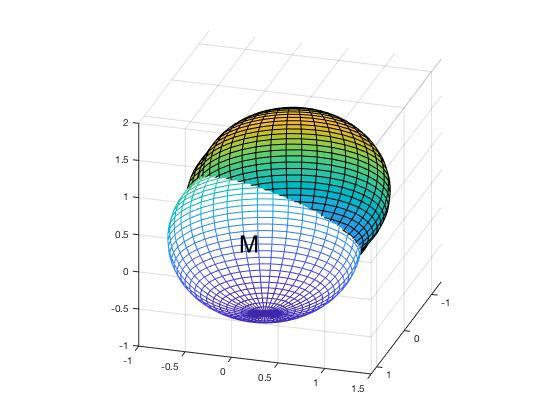
\includegraphics[width=3in]{spheres}}
\end{figure}
Thus if we know $k_g$ (the geodesic curvature) of the boundary of $M$ at all points, we can compute $A$. If $\partial M$ is piecewise smooth, then $\int_{\partial M} k_g ds$ is the sum of the integrals along the components of the boundary plus the sum of the angles by which the elements of the boundary turn at the corners. For the simple example of a geodesic triangle on a sphere of radius $\rho$, $\int_\gamma k_g ds=0$ where $\gamma$ is a piece of $\partial M$. Thus $\int_{\partial M} k_g ds=0+\sum (\pi-\alpha_i)$, where $\alpha_i$ are the interior angles of the triangle. Plugging this into $(5)$ gives $A=\rho^2(-\pi+\sum\alpha_i)$. This is the well known Girard's Theorem. 

In our case, the boundaries of $M$ won't be piecewise geodesic, and thus calculating $\int_{\partial M} k_g ds$ will require knowledge of the circles of intersection between the spheres. With that data calculating $k_g$ simply requires some vector calculus$^1$.
We can calculate the SASA of the entire protein this way, by adding up the contributions of the individual regions $M$ across all atoms.

\section{The Power Diagram Model}
\subsection{Model Assumptions}
As has already been explained and will be mentioned later on, one of the biggest assumptions made is by representing each atom as a ball. This ball is surrounded by a sphere whose distance from the edge of the ball represents the radius of a solvent sphere (Figure 3). A solvent refers to a liquid the molecule is suspended in, usually water. This solvent is being represented continuously rather than as a collection of atoms.
\subsection{Power Diagrams}

Our protein can be represented as a set of atom centers $S$ in $\R^3$ with their corresponding balls of various radii. One aspect of the model is computing the power diagram of this protein. The power diagram is a generalized Voronoi diagram, where instead of the normal Euclidean metric, the definition for distance between an atom with center $z_i$ and radius $\varrho_i$ and a point $x$ is $\pi_i(x)=\|x-z_i\|^2-\varrho_i^2$. This becomes the default Voronoi diagram of $S$ if all the radii are equal. After this power diagram is generated we can associate each set of atoms $S_i$ with its corresponding power cell $P_i$ defined by
\begin{equation*}
P_i=\{x\in\R^3\mid\pi_i(x)\leq\pi_j(x),\forall j\}
\end{equation*}
Each $P_i$ is convex, and together they cover all $\R^3$ without overlap. The dual of this power diagram is a weighted Delaunay Triangulation of $S$ into a set of simplices, or triangles and tetrahedrons. We can compute the surface area of these balls using Delaunay triangulation, which will help us in the later sections. There are additional rules for constructing Delaunay triangles, but for the purposes of this paper, it is only necessary to know how they are constructed from the atoms. 

\begin{comment}
To draw the Delaunay triangles, the centers of the balls are taken to be the vertices of the triangles. If any two circles have adjacent power cells, an edge will be drawn between them. Every three power cells with a common edge will make up a triangle and a tetrahedron will comprise four power shells with a common vertex. There are additional rules for constructing Delaunay triangles, but for the purposes of this paper, it is only necessary to know what the vertices of each triangle represent.
\end{comment}

\begin{comment}
Before launching into how the authors modeled and derived area equations for computational molecular modeling, we should discuss the concept behind $\alpha$-shapes.  $\alpha$-shapes are the foundation of this model, and knowing what they are will help us better understand the derivations presented in the further sections. Hence imagine a set of points in $\R^3$ and we want to describe the 'shape' of these points. One solution is the convex hull of these points, which has been quite well studied. However $\alpha$-shapes are hulls that still include all points, but so so in finer detail than the standard convex hull. Constructing an $\alpha$-shape can be thought of via the following analogy from Fischer\cite{Fischer}.

Imagine a mass of $M\&M$ ice cream in $\R^3$, with a point set $S$ suspended in it like a set of $M\&M$'s. Using a spherical ice cream scoop with radius $\alpha$, we start removing all parts of ice cream we can reach without removing the $M\&M$'s. This includes internal scoops that might not be reachable from the outside. The remaining mass will be an $\alpha$-shape of the set of $M\&M$'s. By varying $\alpha$ from 0 to $\infty$, the corresponding $\alpha$-shape goes from $S$ itself to the standard convex hull of $S$. Convex hulls and $\alpha$-shapes are important because the Delaunay Triangulation of a set in $\R^n$ can be viewed as the projection of the corresponding convex hull in $\R^{n+1}.^3$ Thus we can find the Delaunay Triangulation of the set of atom centers by calculating the convex hull. This computation is also quite fast.
\end{comment}

\begin{comment}
Alpha Shapes are a subset of Delaunay Triangulation, a method that separates a surface into a series of triangles in order to make it easier to identify properties of an object. Alpha-Shapes are more generally known as being comprised of many such triangles, or simplexes. Using Alpha Shapes makes studying three-dimensional balls in space (or molecules) much easier. It provides a way to run computations faster, especially when given large amounts of data. Molecules like proteins are often made with hundreds or thousands of three-dimensional balls, so using the Alpha Shapes method is very practical for these purposes. 

The dual of this Delaunay Triangulation is called the Voronoi Diagram of the atom centers.
The term “Voronoi diagram” is often used to classify the partition of a plane. Each partition is referred to as a “Voronoi cell” (Edelsbrunner). In his paper, Edelsbrunner uses the term “Voronoi cells” to describe each d-ball in $R^3$ (or 3-ball), which has a center z with some point x. The authors describe the atoms as being surrounded by a solvent sphere, which will be elaborated in the next section. Briefly, this model is represented by several terms. First, the power distance of x from b is
\\$\pi_i(x) = ||x-z_i||^2 - (\varrho)^2 $
\\The power distance is the distance from some point in the ball to the solvent shell. The power cell is what minimizes this distance between the point and the solvent shell.
\\$P_i = {x \epsilon \R^3 | \pi_i(x) <= \pi_j(x) \forall j}$
\\All of these spheres, or the alpha-shape, are what’s known as a power diagram. 
\end{comment}

\subsection{Application to Protein Structures}
\begin{comment}
To represent the entire state of the protein (with $n$ atoms) we use the $m=3n$ dimensional  vector \textbf{z}, where consider a set of balls $B_i$ defined by a center $z_i$ and a fixed radius $\varrho_i$ to be in some state \textbf{z} in $\R^{3n}$. Each ball $B_i$ is surrounded by a sphere $S_i$ in this state. It is stated that if any space in $\R^m$ can be approximated by a linear space ($\R$), it is possible to find its derivative. By considering this differentiable map f, which takes the object from $\R^m$ to$\R$, they use this reasoning to say that the derivative of this map is linear. Thus, the authors show that it can be represented by vectors known as \textbf{t} and \textbf{u}, both of which are in $\R^m$, where \textbf{t} is a some variable vector and \textbf{u} is a gradient vector that shows how it changes with \textbf{t}. So the derivative of f will map each \textbf{z} to its gradient, or direction vector. The paper considers a space of $\R^3$ to better represent atoms. It states that m = 3n (so the balls are in $\R^{3n}$), and i can be no less than n-1. So, for some \textbf{z} or $B_i$, the center of $B_i$($z_i$) is stated as $(textbf{z}_{3i+1},textbf{z}_{3i+2},textbf{z}_{3i+3})$. The radius of $B_i$ is noted to be $\varrho_i$.
\end{comment}

Consider a set of balls $B_i$ defined by a center $z_i$ and a fixed radius $\varrho_i$ to be our protein. To represent the entire state of the protein (with $n$ atoms) we use the $m=3n$ dimensional  vector $\textbf{z}\in\R^{3n}$ where $\lbrack{\bf z}_{3i+1}, {\bf z}_{3i+2}, {\bf z}_{3i+3}\rbrack^T=z_i$. Now we can define the weighted and unweighted surface areas $E,A:\R^{3m}\rightarrow\R$ as real multivariate functions from the state of the protein to a single value (the solvent exposed surface area). The weighted area will be described below. Here we will describe the gradients of these maps, written as $DE_{\bf z}$ and $DA_{\bf z}$ which would allow us to calculate SASAs for protein structures and approximate how the SASA changes as the atomic coordinates move. These derivatives map each point in $\R^m$ to a corresponding gradient vector that we call \textbf{u}.


\begin{figure}[h!]
\caption{$B_1$ is bound by a sphere. The radius of the solvent is the distance between the edge of the ball and the sphere.}
\centerline{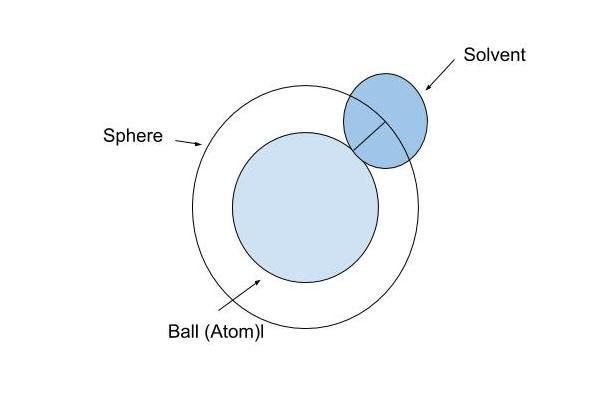
\includegraphics[width=3in]{Figure8}}
\end{figure}

Given a collection of atoms, there will be many overlapping spheres in $\R^{3n}$. We will describe area derivative equations for groups of two or three overlapping spheres, which can easily be applied to larger systems. Using the power method described above, we will show how the authors use Delaunay Triangulations to assist with the calculations.

\begin{figure}[h!]
\caption{Three balls in space bounded by three different spheres. Their centers are used for Delaunay Triangulation.}
\centerline{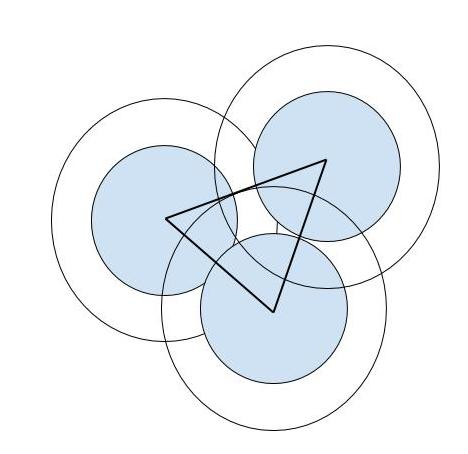
\includegraphics[width=2in]{Figure2}}
\end{figure}

%The authors make use of a power diagram for their model, which is another name for the structure of spheres shown in Figure 2. Just like we mentioned previously, the power diagram consists of power cells. [Repetitive]

\begin{figure}[h!]
\caption{A power diagram comprised of power cells (left) and its Delaunay Triangulation (right).$\lbrack1\rbrack$}
\centerline{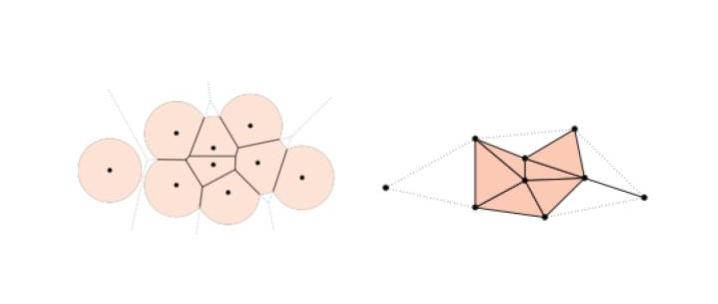
\includegraphics[width=4in]{Figure4}}
\end{figure}


In order to derive the SASA equations, we must define some additional terms. After constructing Delaunay Triangles from a set of molecules, the “star” and “link” of the alpha shape's subcomplex are defined. Each of the Delaunay triangles is a simplex. $K$ is defined as a dual complex, or subcomplex of the alpha shape.

\begin{figure}[h!]
\caption{The dual complex ($K$) of the Delaunay Triangulation only includes those power cells that have a non-empty intersection.$\lbrack1\rbrack$}
\centerline{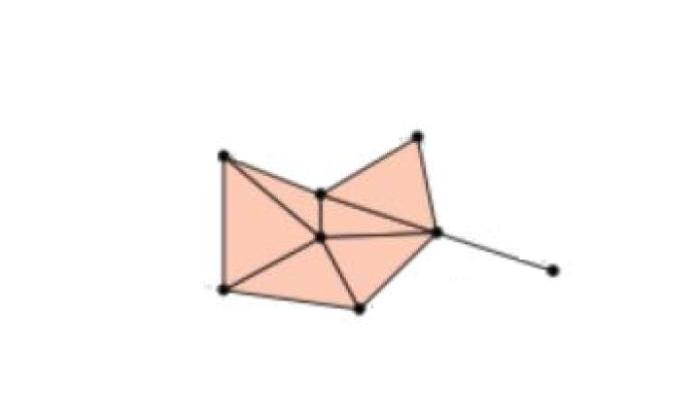
\includegraphics[width=3in]{Figure9}}
\end{figure}

As can be seen by Figure 6, $K$ is made up of multiple simplices. The star of $K$ is a set of triangles who share a vertex and outside boundary. The link of $K$, then, is all of the vertices and edges in the star (Figure 7).

\begin{figure}[h!]
\caption{The star of $K$ and link of the star are shown.$\lbrack1\rbrack$}
\centerline{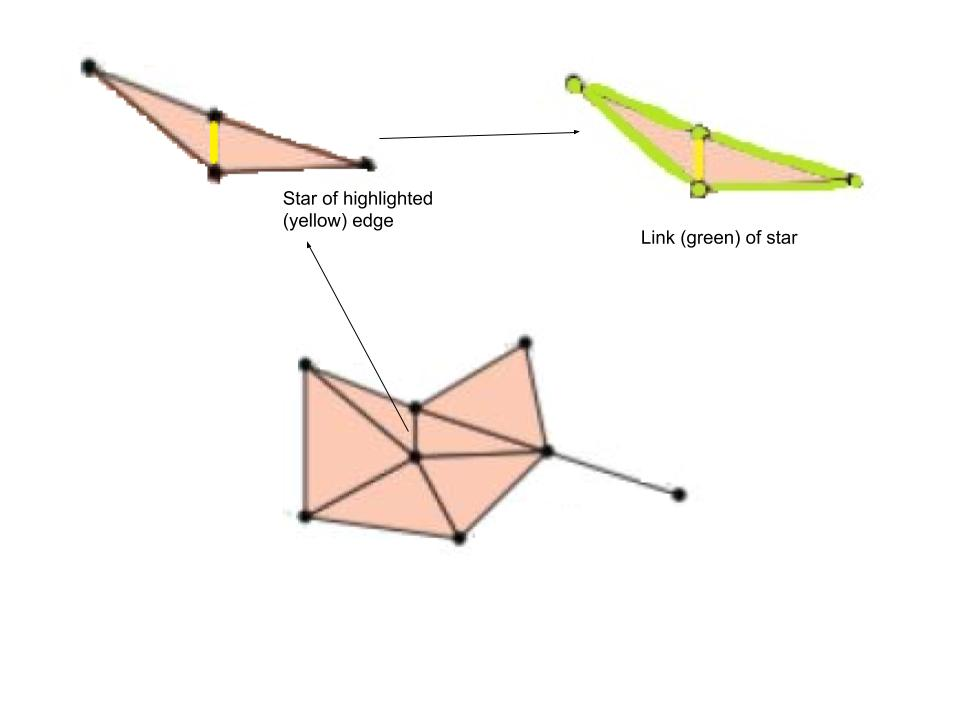
\includegraphics[width=3in]{Figure5}}
\end{figure}

Knowing how the star and link of a subcomplex $K$ are defined is useful when deriving the SASA equations.
The collection of spheres, or the entire molecule, is known as a space-filling diagram $F$. $F_i$, for instance, consists of all the atoms in $S_i$. $\sigma$ represents the fraction of a sphere on the boundary of $F$. We only really care about the boundary of $F$ because that is what contributes to the exposed surface area that will be interacting with the solvent. As mentioned earlier, a molecule can contain multiple spheres that overlap. For two intesecting spheres $S_i$ and $S_j$ that share a circle $S_{ij}$, $\sigma$ comes out to:

\begin{equation}
\sigma_{ij} = \frac{length(P_i \cap P_j \cap bd F)}{length(S_{ij})}
\end{equation}

bd $F$ means the boundary of $F$. This equation shows that for the space-filling diagram of the two intersecting spheres, $\sigma_{ij}$ is the fraction of the exposed surface that's on the power cells of both of the spheres.
Using the dual complex, we can further specify the equation for $\sigma_{ij}$ in terms of two intersecting circles, which will become useful later:

\begin{equation}
\sigma_{ij} = 1 - \frac{\sum_{k}length(S^k_{ij})- \sum_{k,l}length(S^k_{ij} \cap S^l_{ij})}{2\pi\varrho_{ij}}
\end{equation}

This equation is derived by looking at Edelsbrunner's (1995) paper. The same two spheres $S_i$ and $S_j$ intersect at $S_{ij}$. However this time, $S^k_{ij}$ and $S^l_{ij}$ are the interesction of $S_{ij}$ with two other spheres in the power diagram. Both  $S^k_{ij}$ and $S^l_{ij}$ minimize the power distance to $S_{ij}$. Looking at the right side term of equation 7, the first sum adds the portion of $S_{ij}$ coming into contact with $S_k$, while the second sum adds the portion of $S_{ij}$ coming into contact with both $S_k$ and $S_l$. Having this second sum ensures we don't underestimate the amount of unexposed area. Dividing the difference of these sums by the circumference of the circle gives the fraction of this unexposed area, so that subtracting this term from 1 gives the fraction of the exposed surface area of $F$.

$\sigma$ is related to the area of the ball, which for a ball with radius $\varrho$ is $4\pi\varrho^2$. Because we only care about the exposed surface area, we need to multiply by $\sigma$, in order to only get the solvent-exposed surface area. We can also define a weighted area, which only differs from the unweighted area equation by the factor of some parameter $\alpha$, which represents some constant atomic solvation parameters that were predefined by Eisenberg and McLachlan (1986). So for just one ball $B_i$:

\begin{align*}
&A = 4\pi\sum \varrho_i^2\sigma_i
&E = 4\pi\sum\alpha_i\varrho_i^2\sigma_i
\end{align*}


Another term, $\beta_{ijk}$, is also used, which is useful when considering the case of three intersecting spheres. When three spheres intersect at two points, there is a line segment passing through them that is represented as $B_{ijk}$. Just like for $\sigma_{ij}$, $\beta_{ijk}$ represents the fraction of points that belong to the edge of $F$ for these three spheres.
\begin{equation}
\beta_{ijk} = \frac{length(P_i \cap P_j \cap P_k \cap bd F)}{length(B_{ijk})}
\end{equation}

A similar expression to $\sigma_{ij}$ is derived for $\beta_{ijk}$, using $B^l_{ijk}$, the portion of the line segment $B_{ijk}$ on a fourth sphere $S_l$. 
\begin{equation}
\beta_{ijk} = 1 - \frac{\sum_{l}length(B^l_{ijk})}{length(B_{ijk})}
\end{equation}
In the right side term of equation 9, the sum adds up the length of the line segment that comes in contact with $S_l$ and divides that by the entire length of $B_{ijk}$ (which is $2\varrho_{ijk}$), giving the fraction of $F$ that is unexposed. By subtracting this term from 1, the fraction of solvent exposed area for the three intersecting spheres is found.

We can think of the sphere as representing how much of the solvent can interact with the atom. 
\begin{comment}
The state \textbf{z} of each ball defines a center and a radius. As stated before, this paper considers that the weighted (E) and unweighted (A) areas are transformations from the space containing z ($\R^{3n}$) to $\R$. Their derivatives at a particular \textbf{z} are linear maps. In other words, the areas are represented by the map f and their derivatives the derivative of f at \textbf{z}.
\end{comment}

Because the area derivatives are linear, they can be broken down into a sum of components. Both unweighted and weighted area derivatives are comprised of two motions, direction preserving and distance preserving, which can be derived separately and summed to get the SASA derivatives.
 
\subsection{Direction Preserving Motion} 
In direction preserving motion, it is assumed that two spheres $S_i$ and $S_j$ bounded with a non-empty intersection are moving straight on the line passing through their centers.
In this case, the space-filling diagram $F$ consits of all the atoms in $S_i$ and $S_j$, in other words $F = B_i \cup B_j$ (Figure 8).

\begin{figure}[h!]
\caption{Two intersecting spheres $S_i$ and $S_j$.\cite{Bryant}}
\centerline{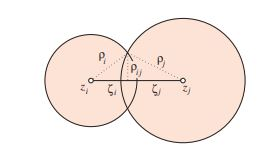
\includegraphics[width=3in]{Figure6}}
\end{figure}


A term $\zeta_{ij}$ is equal to  $\zeta_i$+$\zeta_j$, or the norm of the distance between the centers of the two spheres $z_i$ and $z_j$. $\zeta$ in this case represents the signed distance of each sphere center to the circle of intersection. Each of the sphere's own radii are defined to be $\rho_i$ and $\rho_j$. First, we can assume coordiates for the spheres based on what we know about their centers:
(0,0,$z_i$) and (0,0,$z_j$).


The general equation of a sphere ($x^2 + y^2 +z^2 = r^2$) can be used to construct equations for $S_i$ and $S_j$:
\begin{align*}
&x^2 + y^2 +(z-z_i)^2 = \zeta_i^2 \\
&x^2 + y^2 +(z-z_j)^2 = \zeta_j^2 \\
&\text{Now we can combine the equations:} \\
&\zeta_i^2-\zeta_j^2 =(z-z_i)^2-(z-z_j)^2=-2z_i +2z_j +z_i^2 - z_j^2\\
& \implies -2z_i +2z_j +z_i^2 - z_j^2 = (\zeta_i)^2-(\zeta_j)^2\\
\end{align*}
Using this logic, we can find the same equation holds true if we consider the set of balls for each sphere (assuming they have they same radii), as they have the same center as the spheres. So:
\begin{align*}
&-2z_i +2z_j +z_i^2 - z_j^2 = \varrho_i^2-\varrho_j^2 \\
&\text{From the above two expressions, we can state that:} \\
&\zeta_i^2-\zeta_j^2 = \varrho_i^2-\varrho_j^2\\
&\text{In the left term, we can factor out $\zeta_i^2-\zeta_j^2$ to get:} \\
&\zeta_i^2-\zeta_j^2 =(\zeta_i-\zeta_j)(\zeta_i+\zeta_j) = \zeta_{ij}(\zeta_i-\zeta_j) \\
&\text{So we can state that:} \\
&\varrho_i^2 - \varrho_j^2  = \zeta_{ij}(\zeta_i-\zeta_j) \\
&\text{Now we can find what $\zeta_i$ and $\zeta_j$ really are} \\
&\varrho_i^2 - \varrho_j^2)/\zeta_{ij} + \zeta_j = \zeta_i \\
&\text{We know that $\zeta_j = \zeta_{ij} - \zeta_i$, so just substitute this expression in:} \\
&\zeta_i = \frac{1}{2}\left(\zeta_{ij}+\frac{\varrho_i^2-\varrho_j^2}{\zeta_{ij}}\right) \\
&\text{A similar statement can be made for $\zeta_j$, following the steps we carried out above:} \\
&\zeta_j = \frac{1}{2}\left[\zeta_{ij}+\frac{\varrho_j^2-\varrho_i^2}{\zeta_{ij}}\right]
\end{align*}

Now we can find the area of both spheres. For two spheres, it makes sense that $A = A_i + A_j$. Recall the area equation stated in Section 3.3. For two balls we can say: $A = 4\pi\varrho^2\sum{\sigma_i} + 4\pi\varrho^2\sum{\sigma_j}$. We have already shown what $\sigma$ is, so we can plug it in and simplify the area equation:
\begin{align*}
&4\pi\varrho_i^2\frac{\varrho_i + \zeta_i}{2\varrho_i} + 4\pi\varrho_j^2\frac{\varrho_j + \zeta_j}{2\varrho_j} \\
&\text{After a few algebraic simplifications:} \\
&2\pi\varrho_i^2 +2\pi\varrho_j^2 +\pi\varrho_i\left(\zeta_{ij} + \frac{\varrho_i^2 - \varrho_j^2}{\zeta_{ij}}\right)+\pi\varrho_j\left(\zeta_{ij} + \frac{\varrho_j^2 - \varrho_i^2}{\zeta_{ij}}\right) \\
&A  = 2\pi(\varrho_i^2 + \varrho_j^2) + \pi(\varrho_i+\varrho_j)\left[\zeta_{ij}+\frac{(\varrho_i-\varrho_j)^2}{\zeta_{ij}}\right] \\
&\text{Finally, we can find the derivative of the area with respect to $\zeta_{ij}$:} \\
&\frac{dA}{d\zeta_{ij}} = \pi(\varrho_i+\varrho_j)\left[1-\frac{(\varrho_i - \varrho_j)^2}{\zeta_{ij}^2}\right] \\
&\text{This is term we get after some simplification.}
\end{align*}

\subsection{Distance Preserving Motion}
In distance preserving motion, one sphere rotates about the other. Imagine three spheres interesting at two points, $p$ and $q$ (Figure 9). This time, $F$ is going to include all the points contained in all three spheres. It is assumed that if the spheres intersect at two points then one sphere contains the other two. In this case, it is $S_j$ that engulfs $S_i$ and $S_k$. The caps, or tops of the spheres, are considered. From a previous section, we know that $B_{ijk}$ is considered the line segment of three intersecting spheres. In this case, $B_{ijk}$ is the line segment containing $p$ and $q$. The caps $C_{ij} = B_i \cup S_j$ and $C_{kj} = B_k \cup S_j$ protrude from the surface of $S_j$. The parameters obtained from this diagram allows us to find the area similar to how we found it for the direction preserving motion. This model says that as you move the two caps apart, keeping their centers in the same position, you will gain an area equal to that of a spherical rectangle. Essentially, the caps are rotating in place. It might be easy to think about how diameter of the caps can represent the height of this “rectangle” while the distance between the caps signifies its width.
\begin{figure}[h!]
\caption{Three intersecting spheres at two points: $S_i$, $S_k$ and $S_j.\lbrack1\rbrack$}
\centerline{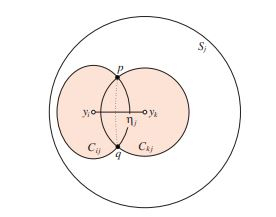
\includegraphics[width=3in]{Figure7}}
\end{figure}

Using this spherical rectangle shape, and the fact that we know the caps are rotating, the change in area is found to be the change in the distance between the center of the circles $\eta_j$ divided by the circumference of the set of balls in the larger sphere (which is $S_j$ in this case) times the area of the slice of $S_j$ between $p$ and $q$: 
\begin{align*}
dA_j = \frac{d\eta_j}{2\pi\varrho_j}4\pi\varrho_j\varrho_{ijk}\\
\end{align*}
$\frac{d\eta_j}{2\pi\varrho_j}$ acts like the change in the “width” of the spherical rectangle while $4\pi\varrho_j\varrho_{ijk}$ serves as the change in the “height” of the spherical rectangle. The area derivative of this larger sphere becomes:

\begin{equation*}
\frac{dA_j}{d\eta_j }= 2\varrho_{ijk}
\end{equation*}

\subsection{Combining the Area Equations}
Now that we've derived area derivative equations for both types of motions, we can see how they’re able to come together. As mentioned before, because the derivatives are linear, they can be separated into a sum of certain components. The gradient vector \textbf{u} shows the direction or trend of the area. For the case of the direction-preserving motion it is stated $u_{ij} = \frac{z_i - z_j}{\zeta_{ij}}$ , showing that the unit vector $u_{ij}$ for two intersecting spheres $S_i$ and $S_j$ is dependent on the distance between their centers. The gradient vector $u_{ijk}$ for distance preserving motion is dependent on the component of the intersection to two of the spheres ($u_{ik}$) that is normal to the component of intersection between the other two spheres ($u_{ij}$). This makes $u_{ijk} = \frac{u_{ik} - <u_{ik},u_{ij}> \cdot u_{ij}}{\|(u_{ik} - <u_{ik},u_{ij}>) \cdot u_{ij}\|}$.

Based on what has already been shown, the unweighted and weighted area derivative theorems can be stated. Remember that we said each state \textbf{z} was in $\R^{3n}$, and each \textbf{z} represents a set of balls $B_i$ so that $0\leq i \leq n-1$. Looking at the area derivative theorem, the derivative of the area at some \textbf{z} is said to be $DA_z(\textbf{t}) = <\textbf{a},\textbf{t}>$, where \textbf{a} is a gradient vector like \textbf{u} and 	\textbf{t} is the variable vector mentioned above. They state that for the unweighted area derivative,
\begin{equation}
\textbf{a} = \sum_j \sigma_{ij}\cdot a_{ij}+ \sum_j \sum_k \beta_{ijk}\cdot a_{ijk}
\end{equation}

The first sum of equation 10 shows the contribution of the direction preserving motion while the second sum shows the contribution of the distance preserving motion. We can see for the first sum that we are summing over all of the points along $F$ in $K$ when considering direction preserving motion for $S_i$ across all $S_j$. Similarly, the second sum considers distance preserving motion for $S_i$ across all $S_j$ and $S_k$ in $K$. From this, $a_{ij}$ and $a_{ijk}$ are:
\begin{align*}
&a_{ij} = \pi(\varrho_i+\varrho_j)\left[1 - \frac{(\varrho_i - \varrho_j)^2}{\zeta_{ij}^2}\right]\cdot u_{ij}\\
&a_{ijk} = 2\varrho_{ijk}\frac{\varrho_i - \varrho_j}{\zeta_{ij}} \cdot u_{ijk}
\end{align*}
$a_{ij}$ and $a_{ijk}$ depend on the unit vectors $u_{ij}$ and $u_{ijk}$, respectively.


The weighted area derivative theorem, defined as $DE_z(\textbf{t}) = <\textbf{e},\textbf{t}>$ is defined similarly to the unweighted area derivative theorem, but multiplied by the solvent parameter $\alpha$:
\begin{align*}
&\textbf{e} = \sum_j \sigma_{ij}\cdot e_{ij}+ \sum_j \sum_k \beta_{ijk} \cdot e_{ijk} \\
&e_{ij} = \pi\left((\alpha_i\varrho_i +\alpha_j\varrho_j) - \frac{(\alpha_i\varrho_i  - \alpha_j \varrho_j)(\varrho_i^2 - \varrho_j^2)}{\zeta_{ij}^2}\right)\cdot u_{ij} \\
&e_{ijk} = 2\varrho_{ijk}\frac{\alpha_i\varrho_i - \alpha_j\varrho_j}{\zeta_{ij}}\cdot u_{ijk}
\end{align*}
Not surprisingly, $e_{ij}$ and $e_{ijk}$ depend on (respectively) $u_{ij}$ and $u_{ijk}$ as well.

Above, we described $\textbf{a}$ and $\textbf{e}$. Using these, we can then clearly state the area derivative equations. For the unweighted area derivative equation, the direction preserving component is the the fraction of the solvent-exposed surface times the derivative of the area: $\sigma_{ij}<a_{ij},t_i>$ and the distance preserving component is the same: $\beta_{ijk}<a_{ijk},t_i>$. We know that the unweighted area derivative is the sum of these two components:
\begin{equation}
DA_z(\textbf{t}) = \sum_{i=0}^{n-1}\sum_{j\neq i}\left(\sigma_{ij}<a_{ij},t_i> + \sum_{k\neq i,j} \beta_{ijk}<a_{ijk},t_i>\right)
\end{equation}
Just like before, the weighted area derivative is basically the same as the unweighted derivative: 
\begin{equation}
DE_z(\textbf{t}) = \sum_{i=0}^{n-1}\sum_{j\neq i}\left(\sigma_{ij}<e_{ij},t_i> + \sum_{k\neq i,j} \beta_{ijk}<e_{ijk},t_i>\right)
\end{equation}

These are the derivative equations that can then be tested on different molecules. It is important to note that there are cases where these equations will be discontinuous. We won't elaborate on these, but, for example, discontinuities can happen in a case where three spheres intersect at a circle. There are other cases of discontinuities, which are useful to know in order successfully to run this algorithm for a variety of molecules.

\begin{comment}
\subsection{Model Assumptions}
As explained above, one of the biggest assumptions made is by representing each atom as a ball. This ball is surrounded by a sphere whose distance from the edge of the ball represents the radius of a solvent sphere (Figure 1). A solvent refers to a liquid the molecule is suspended in, usually water. Another assumption to point out is that water is being represented as a sphere (continuously) rather than a collection of atoms. 
\end{comment}


\section{Application of ALPHAMOL to Molecular Modeling}
To test the time cost of \textsc{alphamol} (the computational implementation of the method described in $\S3$) versus the Shrake-Rupley Algorithm we took 100 PDB structures from the RCSB\cite{PDB} database (listed in the supplemental) with between 30 and 330 residues and directly calculated surface areas using PyRosetta\cite{Chaudhury}, a python wrapper for Rosetta that allowed us to write a script that computed SASA for 100 structures using these two methods. We measured the time to compute SASA for each PDB for each method, and plotted this data against residue count. It can be seen that the \textsc{alphamol} method is substantially slower than the Shrake-Rupley method and that the time cost of both increases roughly linearly with the size of the structure, though it is clear that \textsc{alphamol} incurs time penalties faster than Shrake-Rupley as the structure size increases.


\begin{figure}
\centerline{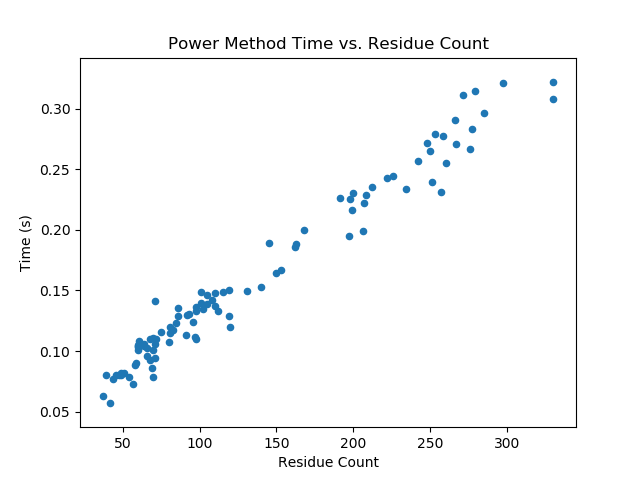
\includegraphics[width=3in]{daltimes}}
\caption{Plot of Computation Time versus Residue Count (Power Method)}
\end{figure}
\begin{figure}
\centerline{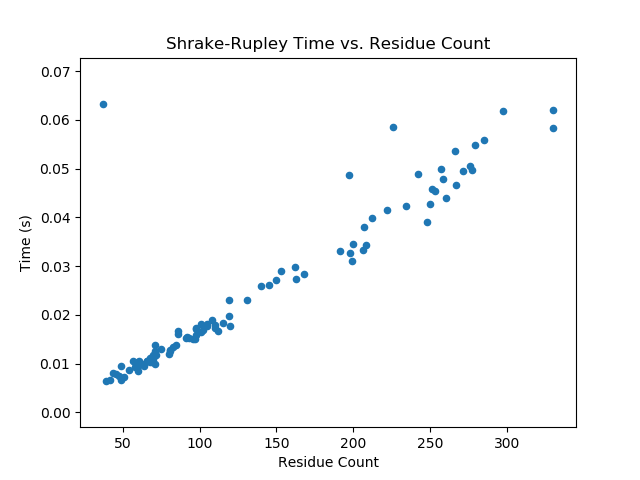
\includegraphics[width=3in]{voxtimes}}
\caption{Plot of Computation Time versus Residue Count (Shrake-Rupley Method)}
\end{figure}

We also plotted the distribution of the SASA values for each calculator, and while the don't look too different in this example, more rigorous testing with a wider range of proteins has shown that \textsc{alphamol} gives far more accurate values than other algorithms, which is why it is incorporated into Rosetta today.
\begin{figure}
\caption{SASA Histograms for the Two Algorithms}
\centerline{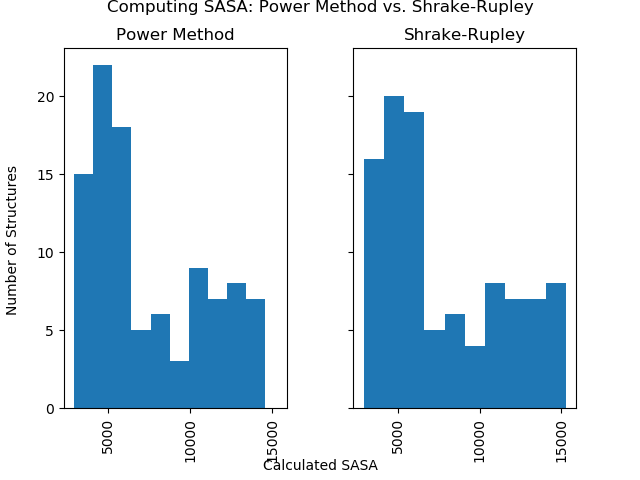
\includegraphics[width=3in]{sasa}}
\end{figure}

\section{Conclusion}
It can be seen that SASA is a critical quantity to be able to compute for the purposes of structural biology. On a per-atom basis, it is one metric that can be used to determine if an atom is making a hydrogen bond, and by extension if the structure is energetically favorable. For protein-protein interfaces, large SASA values at the interface usually mean the proteins are more likely to bind because there is a larger binding surface. Metrics like SASA are useful because they don't require your structure to look similar to any existing PDB in order to determine if the structure is likely to be stable. This is especially important in the field of protein engineering, where there might not be any structures to compare your PDB to, and thus having independent metrics is critical to filtering out possible \textit{de novo} protein designs from sequences that won't take on any definite conformation. Thus much time has been spent on applying mathematical and computational ideas to rigorously defining and calculating SASA, in this paper we have explored a few of the most prominent methods.

\section{Glossary}
\begin{align*}
&\varrho_i:&\text{The radius of ball i} \\
&z_i:&\text{The center of a ball i} \\
&{\bf z}:&\text{The $3n$ dimensional vector representing the state of all $z_i$} \\
&\zeta_{ij}:&\text{The signed distance between centers of two intersecting spheres} \\
&\sigma_{ij}:&\text{The fraction of solvent-exposed surface for two intersecting spheres $S_i,S_j$} \\
&\beta_{ijk}:&\text{The fraction of solvent-exposed surface for three intersecting spheres $S_i,S_j, S_k$} \\
&\alpha:&\text{An atomic solvation parameter} \\
&F:&\text{The space filling diagram} \\
&\pi_i(x):&\text{The power distance of a random point x from $S_i$} \\
&P_i:&\text{The set of points closer (by power distance) to $S_i$ than any other sphere} \\
&K:&\text{The dual complex of Delaunay Triangulation. Consists of all power cells with non-empty intersection} \\
&DA_{\bf z}({\bf t}):&\text{The unweighted area derivative at \textbf{t}} \\
&DE_{\bf z}({\bf t}):&\text{The weighted area derivative at \textbf{t}} \\
\end{align*}

\section{Supplemental Information}
List of PDB's used: \\
1W4H, 2FD7, 1I2U, 1HA8, 1RO3, 1FRE, 1AHL, 1B8W, 1B7I, 3UA6,\\
1B7K, 1IVA, 1L6H, 1KTH, 2GQV, 2KXK, 1CDT, 1BF0, 1B7V, 4AEI,\\
4BWS, 1UBQ, 1FGP, 1CPZ, 1B4R, 1CRE, 2BCB, 4ZK9, 1BCG, 1B3C,\\
1G47, 1NEI, 1HYM, 1A7H, 1COU, 4W9A, 1A70, 1EMV, 1AVS, 1QYS,\\
1BB8, 1HA6, 2HSH, 2ACY, 1THX, 2Z9H, 2CBM, 2APB, 2FLS, 1AIU,\\
4DZN, 1SRR, 2GZV, 2XKH, 1RKI, 1BMG, 2MCT, 1FI5, 1WOU, 1DZO,\\
1DC9, 5PC4, 1WDV, 2OXZ, 1P3B, 129L, 4FH1, 1S2B, 2R32, 1BWR,\\
6MKL, 3CS1, 3PMD, 2O35, 3S9B, 3PFC, 2CA8, 2EBY, 1IIB, 1GAJ,\\
1I9Q, 4LUP, 3RQ8, 1VHI, 5OIL, 6CW0, 2YM4, 2ZO1, 4KXO, 6G0M,\\
5R2D, 2GNP, 6F65, 2CM8, 5OH3, 2W5L, 2VV9, 6CQS, 6DJA, 6D40.

PyRosetta Code:
\lstinputlisting[language=Python]{sasa.py}

\begin{thebibliography}{10}

\bibitem{Bryant} 
Bryant, R, Edelsbrunner, H, Koehl, P, Levitt, M. The Area Derivative of a Space-Filling Diagram. Discrete \& Computational Geometry. 32 (2004), 293-308.

\bibitem{DeCoste}
DeCoste, Donald J, Zumdahl, Steven S. General Chemistry 142 University of Washington 7th Edition, Boston, Cengage Learning, 2015.

\bibitem{Edelsbrunner} 
Edelsbrunner, H. The Union of Balls and Its Dual Shape. Discrete \& Computational Geometry. 13 (1995), 415-440.

\bibitem{Fischer} 
Fischer, Kaspar. Introduction to Alpha Shapes. Stanford University, lecture notes, 2011.

\bibitem{Le Grand}
Le Grand, Scott M, Merz, Kenneth M. Jr. Rapid approximation to molecular surface area via the use of Boolean logic and look-up tables. Journal of Computational Chemistry. 14 (1993). 349-352.

\bibitem{PDB} 
H.M. Berman, J. Westbrook, Z. Feng, G. Gilliland, T.N. Bhat, H. Weissig, I.N. Shindyalov, P.E. Bourne.
(2000) The Protein Data Bank Nucleic Acids Research, 28: 235-242.

\bibitem{Richmond}
Richmond, Timothy J. Solvent Accessible Surface Area and Excluded Volume in Proteins. J. Mol. Biol. 178 (1984), 63-89.

\bibitem{Rotskoff}
Rotskoff, Grant. The Gauss-Bonnet Theorem. University of Chicago REU, paper, 2010

\bibitem{Chaudhury}
S. Chaudhury, S. Lyskov \& J. J. Gray, "PyRosetta: a script-based interface for implementing molecular modeling algorithms using Rosetta," Bioinformatics, 26(5), 689-691 (2010).

\bibitem{Schnell}
Schnell, Christian. The Gauss-Bonnet Theorem. talk at Columbus, 2004.

\end{thebibliography}

\listoffigures
\end{document}  
